\subsection{zkLedger}
zkLedger \cite{zkLedger} is a permissioned, fully-private payment system that supports auditing by a general auditor. It succeeds to provide strong transaction privacy properties, such as hiding the transfered amounts, the participants as well as the link between the transactions (transaction graph), while allowing an auditor to compute provably correct functions over the on-chain data. Audit procedure takes place as an interactive protocol between the users and an auditor, where the latter queries the former about its contents on the ledger. 

Since an auditor cannot distinguish the participants of a transaction, zkLedger should ensure that during auditing a user cannot leave out transactions that participated, in order to be able to receive reliable answer to its queries.

The solution, that zkLedger proposed, to this problem relies on its unique ledger. That is, a table where transactions correspond to rows, and Users (Banks) correspond to columns. Each transaction include information for all other users, even for those who do not participate. To hide the transfered amounts as well as the assets each user holds each entry in a transaction are contains a commitment to a value that is debited or credited to the user. All entries for the non-participants are a commited value to 0 (\autoref{fig:zkLedger-table}). Due to the hiding property of the commitments an adversary cannot distinguish between a zero and a non-zero commited value.

\subsubsection{Transactions}
The transactions in zkLedger are publicly verifiable and must satisfy the following invariants:
\begin{itemize}
    \item Transactions conserves assets, meaning a transfer transaction cannot create or destroy assets.
    \item The spending user gives concent to the transfer and actually own enough assets to execute the transaction.
    \item After each transactions all users have enough information to open their commitments for the audit functionality.
\end{itemize}

Therefore, transactions are formed via a combination of commitments and the zero-knowledge proofs and have the following form $\txn = (cm_i, Token_i, \pi^B, \pi^A, \pi^C)$:
\begin{itemize}
    \item \textbf{Commitment ($cm_i$)}: $(g^{v_i}h^{r_i})$ a Pedersen commitment to the transfered value.
    \item \textbf{Audit token ($Token_i$)}: $(pk_i)^r_i$ used in order to enable user to create reliable answers to the audits without knowing the randomness used in the commitment.
    \item \textbf{Proof of balance ($\pi^B$)}: a zero-knowledge proof asserting the preservation of balance in each transaction $\sum_{k=1}^n v_k = 0$.
    \item \textbf{Proof of assets ($\pi^A$)}: a zero-knowledge proof asserting that the sender has the assets to transfer. In zkLedger a column in the ledger represents all the assets the corresponding user has received or spent. So $\pi^A$ is proven by creating a commitment to the sum of values for the asset in its column, including the current transaction. If the sum is greater than or equal to 0, then the user has the right to transfer the amount. 
    \item \textbf{Proof of consistency ($\pi^C$)}: a zero-knowledge proof asserting that a malicious user cannot add  data to the ledger that would prevent another user to be able to open their commitments.
\end{itemize}

Finally, whenever a transactions happens, a new row is added to the ledger.

\begin{figure}
    \centering
    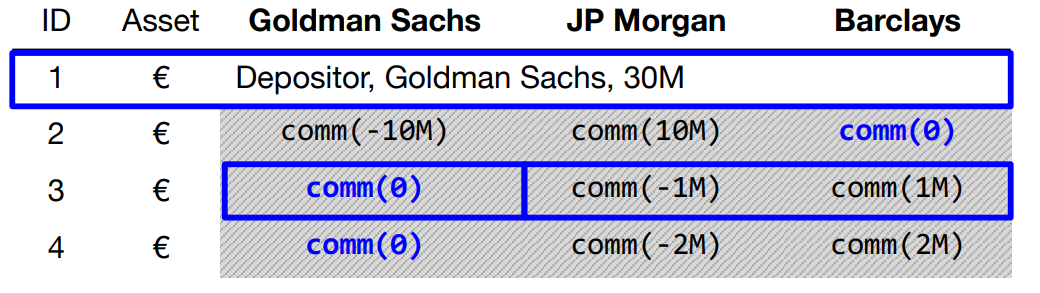
\includegraphics[width=0.9\textwidth]{images/zkLedger/zkledger.png}
    \caption{zkLedger Ledger - naive transaction example}
    \label{fig:zkLedger-table}
\end{figure}

\subsubsection{Auditing}

The Auditor has access to the ledger and interact with the users to calculate functions on their private data. This functions allow the auditor to issues queries that includes information about ratios of holdings, sums, average, variance, outliers, changes over time. The account holder reveal only the value hidden in commitment necessary for the question, without leaking any other information. However, frequent auditing is possible to reveal more of a transaction contents.

\autoref{fig:zkLedger-audit} illustrate an example. An auditor can ask a user "How many euros do you hold at time $t$?". The user responds with an answer along with the validity zero-knowledge proof. The auditor can multiply all the commitments on the ledger for the audited user and can verify if the proof and the answer are valid. Since each column of the ledger represents all the assets that the corresponding user has received or spent, the auditor can be sure that user could not hide any of their transaction during the audit.

\begin{figure}
    \centering
    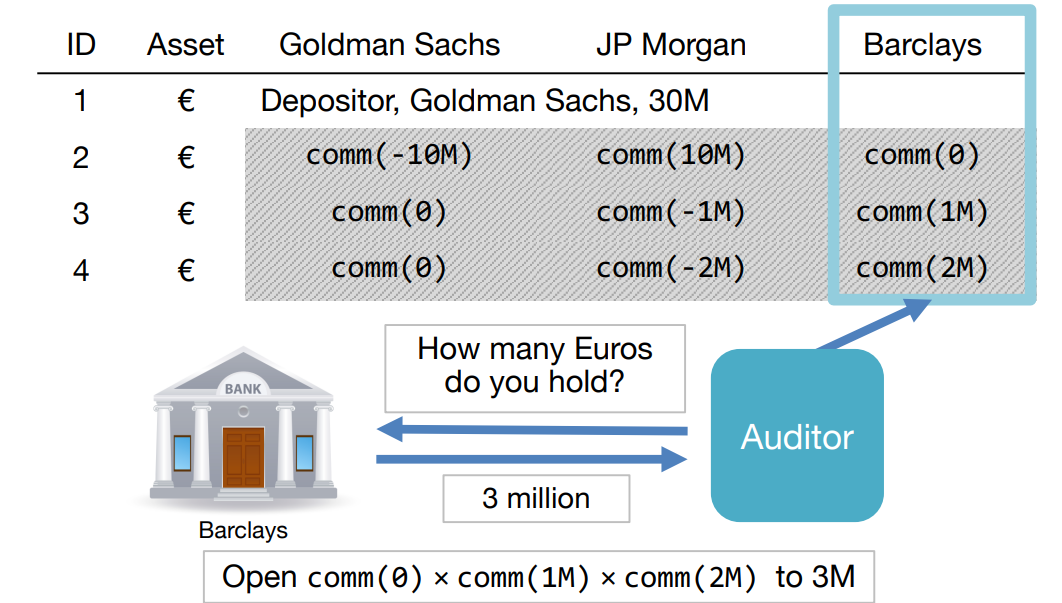
\includegraphics[width=0.9\textwidth]{images/zkLedger/zkledger-audit.png}
    \caption{zkLedger - audit functionality example}
    \label{fig:zkLedger-audit}
\end{figure}

\subsubsection{Setbacks}
Although zkLedger combines full privacy with auditability and offers a wide variety of audit functionalities, suffers from very limited scalability. There are two significant costs that grow with the number of users. The verification of transactions which increases with the number of the users as well as The sequential steps to create transactions increase linearly. 

Considering the verification, zkLedger requires each transaction to include commitments and zero-knowledge proofs for all users. This fact, combined with the ever-increasing ledger that grows with every transaction, results in large computational and storage costs. To overcome this problem an improvement of zkLedger protocol has been proposed called miniLedger \cite{MiniLedger}.

Concerning the second setback, in order a user to be able to produce a new transaction (for exmample transaction $n$) they must use the state of the ledger right before, meaning the must known the $n-1$ transaction. Therefore, multiple users cannot produce different transactions in parallel, since concurrent transactions always have conflicts.